\section{Auswertung}


    \subsection{Widerstand}


    Das Außmessen der Proben ergibt:
    \begin{table}[H]
        \centering
        %\caption{Die Messwerte}
        \begin{tabular}{ S  S [table-format=1.5] S [table-format=1.4] S [table-format=1.6] S [table-format=1.6] S [table-format=1.2]}
            \toprule
            {Metall} & {Höhe}& {Breite}& {Dicke}& {Durchmesser} & {Länge}\\
            \midrule
            \text{Zink} & 0.02603  & 0.0280 & 0.000430 & 0.000263 & 1.73\\
            \text{Kupfer} & 0.04406  & 0.0253 & 0.000018 &  0.0001052 & 1.73\\
            \bottomrule
        \end{tabular}
    \caption{Eine Tabelle zu den Dimensionen der Metall-Proben in $\si{\centi\metre}$.}
    \label{tab:Dimensionen}
    \end{table}

    \noindent Die Messwerte zur Höhe, Breite und Dicke beziehen sich hier auf die Metallplatte, die Messwerte zum Durchmesser und zur Länge
    beschreiben das jeweilige Kabel zur Berechnung des Widerstandes. Hier gehen wir jeweils von einer Ungenauigkeit von einem Prozent 
    des jeweiligen Messwertes aus.\\
    \noindent Der Widerstand eines Metalls berechnet sich mittels: 
    
    \begin{equation}
        U = R \cdot I
    \end{equation}
    \noindent
    Die Berechnung des Widerstandes gibt eine Reihe an Widerständen \ref{tab:ErgWider}, der Mittelwert dieser Reihen ergibt dann einen Widerstand 
    für Zink und Kupfer:

    \begin{align}
        R_{\text{Zink}} &= \SI{13.68+-0.23}{\milli\ohm}\\
        R_{\text{Kupfer}} &= \SI{7.73+-0.05}{\milli\ohm}
    \end{align}

    Der spezifische Widerstand eines Metalls berechnet sich nun mittels der Formel

    \begin{equation}
        \rho = \frac{RA}{l}
    \end{equation}
    \noindent
    mit $R$ dem Widerstand, $A$ der Querschnittsfläche und $l$ der Länge des Kabels.
    Somit ergibt sich mit denn Werten aus \ref{tab:Dimensionen} und den berechneten Widerständen der spezifische Widerstand:

    \begin{align}
        \rho_{Zink} &= \SI{1.72+-0.05}{\nano\ohm\meter}\\
        \rho_{Kupfer} &= \SI{0.16+-0.31}{\nano\ohm\meter}
    \end{align}


    \subsection{Hall-Effekt}

    

    In den folgenden Plots ist sind die Messergebnisse der Hallspannung, mit denen die weiteren Rechnungen ausgeführt werden, 
    aufgetragen. Die Zahlenwerte sind hier \ref{tab:messHall1},\ref{tab:messHall2},\ref{tab:messHall3},\ref{tab:messHall4} zu finden.
    

    \begin{figure}[H]
        \centering
        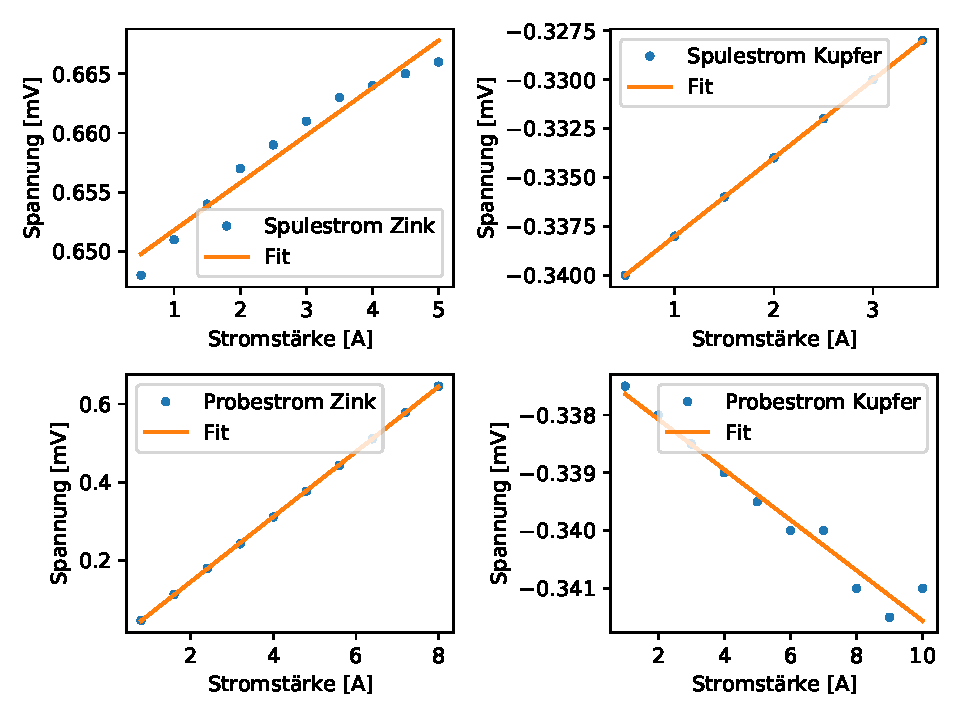
\includegraphics[width=1.1\textwidth]{build/Hall.pdf}
        \caption{Ein Plot der Hall Spannungen gegen die Stromstärke.}
        \label{img:messHall}
    \end{figure}
    
     
    \subsection{Ladungsträger pro Volumen}


    Zur Berechnung der Elektronendichte wird zunächst das Magnetfeld der Spule in Abhängigkeit von der Stromstärke bestimmt.

    \begin{figure}[H]
        \centering
        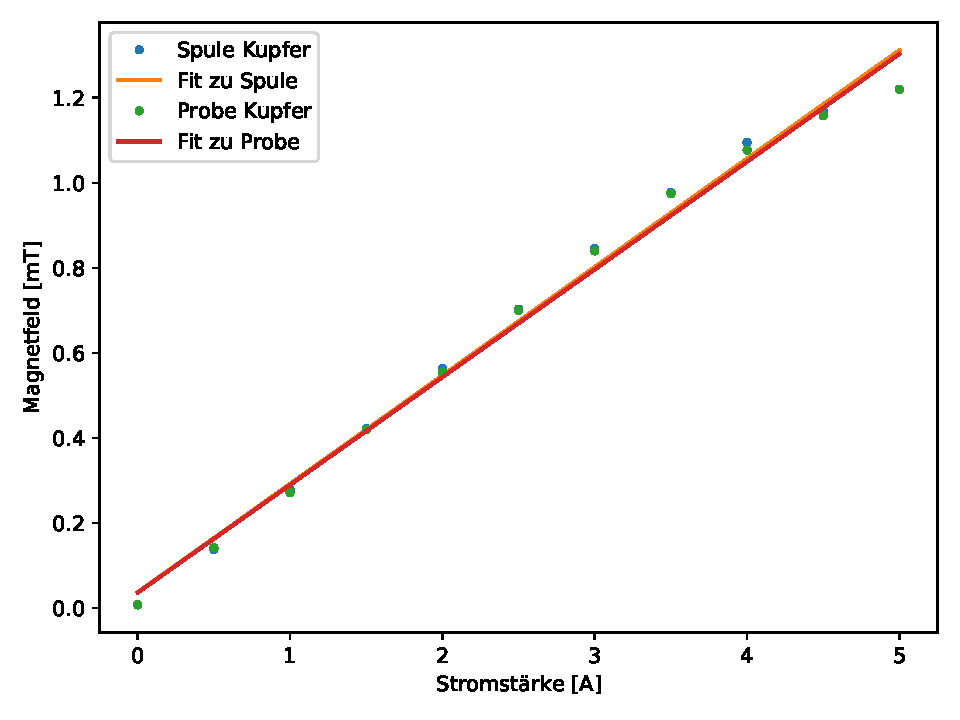
\includegraphics[width=0.7\textwidth]{build/Magnetfeld.pdf}
        \caption{Ein Plot der Magnetfeldstärke gegen die Stromstärke.}
        \label{img:Magnetfeld}
    \end{figure}
    \noindent
    In diesem Plot sind die Magnetfelder bei steigender und abfallender Stromstärke \ref{tab:messMag} und der jeweilige lineare Fit zu den 
    Messwerten eingezeichnet.
    Die Ausgleichsgerade der Form $\text{a}\cdot x = \text{b}$ hat dann die Werte:
    \begin{align}
        \text{a} & = \num{254(5)e-3}\\
        \text{b} & = \num{36.750(16)e-3}
    \end{align}
    In allen folgenden Rechnungen gibt diese Funktion nun einen Wert für das Magnetfeld, wenn nur ein Wert für den Spulenstrom bekannt ist.

    \noindent
    Aus der Formel \ref{eqn:uhall} lässt sich nun eine Formel für die Ladungsträger pro Volumen herleiten:
    \begin{align}
        n &= \frac{-BI}{Ud\cdot\text{e}_0}
    \end{align}
    hier ist $B$ der magnetischen Feldstärke, $I$ der Stromstärke, $U$ der Hall-Spannung, $d$ der Dicke der jeweiligen Proben und $\text{e}_0$ der 
    elementar Ladung.
    \noindent
    Mit den angegeben Messwerten lässt sich nun die Elektronendichte pro Volumen bestimmen. Dies findet man in den nachfolgenden Plots:
    \begin{figure}[H]
        \centering
        \includegraphics[width=1.1\textwidth]{build/N.pdf}
        \caption{Ein Plot der Elektronendichte gegen die Stromstärke.}
        \label{img:elekdichte}
    \end{figure}
    \noindent
    Die durch die Plots veranschaulichten Werte sind auch in der Tabelle \ref{tab:Ergn1},\ref{tab:Ergn2} zu finden.


    \subsection{Ladungsträger pro Atom}


    Die Anzahl der Atome pro Volumen berechnet sich mittels der Formel:
    \begin{equation}
        \frac{\text{Atome}}{\text{V}} = \frac{\rho \cdot \symup{N_A}}{\symup{m_{mol}}}
    \end{equation}
    Mit $\rho$ der Dichte des Metalls, $\symup{N_A}=\SI{6.02214076e23}{\per\mole}$ der Avogrado-Konstante und $\symup{m_\text{mol}}$ der 
    molaren Masse des Metalls.
    Aus dieser Formel ergibt sich direkt die Formel für Z, die Anzahl der Ladungsträger pro Atom:
    \begin{equation}
        Z=\frac{n \cdot \symup{m_{mol}}}{\rho \cdot \symup{N_A}}
    \end{equation}
    Mit den stoffspezifischen Größen
    \begin{table}[H]
        \centering
        %\caption{Die Messwerte}
        \begin{tabular}{ S  S [table-format=1.5] S [table-format=1.4] }
            \toprule
            {Metall} & {$\rho [\si{\gram\per\mole}]$}& {$\symup{m_{mol}}[\si{\gram\per\mole}]$}\\
            \midrule
            \text{Zink} &  7.14 & 65.38 \\
            \text{Kupfer} & 8.92 & 63.55 \\
            \bottomrule
        \end{tabular}
    \caption{Eine Tabelle mit stoffspezifischen Größen der Metalle.}
    \label{tab:spez}
    \end{table}
    \noindent
    lässt sich nun Z berechnen. In den folgenden Plots ist Z für die unterschiedlichen Messreihen angegeben.
    \begin{figure}[H]
        \centering
        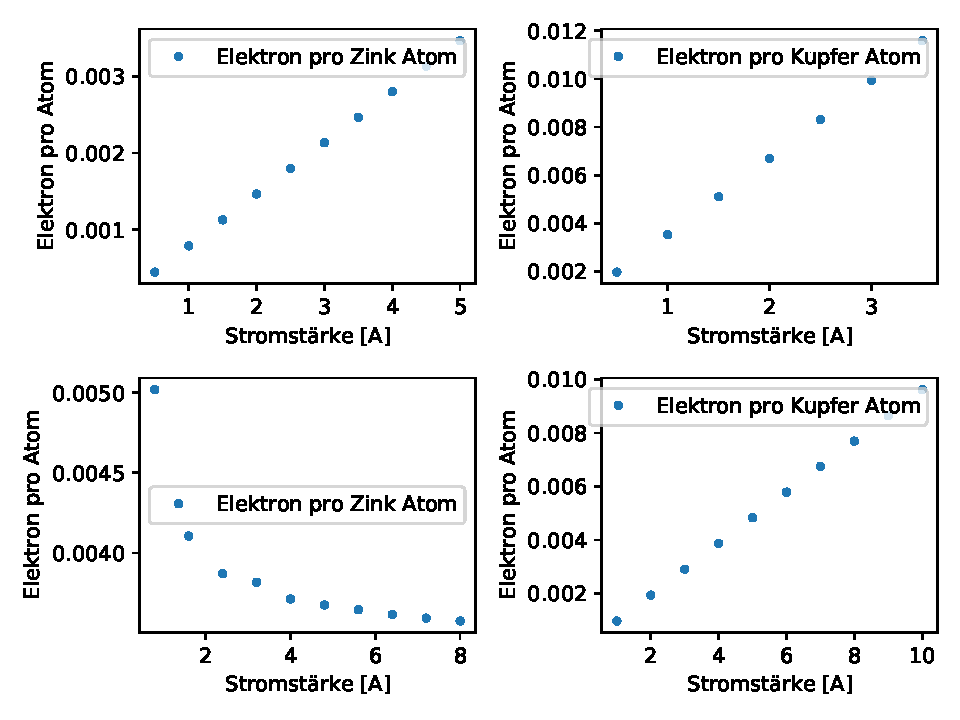
\includegraphics[width=1.1\textwidth]{build/Z.pdf}
        \caption{Ein Plot der Elektronendichte gegen die Stromstärke.}
        \label{img:elekZahl}
    \end{figure}
    \noindent
    Die zugehörigen Ergebnisse sind auch wieder in den Tabellen \ref{tab:ErgZ1},\ref{tab:ErgZ2} zu finden.


    \subsection{Mittlere Flugzeit}

    
    Die Formel \ref{eqn:rho} wir so umgestellt, dass wir folgende Formel erhalten:
    \begin{equation}
        \overline{\tau} =\frac{2}{n}\frac{\symup{m_0}}{\symup{e_0}^2 \cdot \rho}
    \end{equation}
    In dieser Formel rechnen wir mit dem Reziproken des spezifischen Widerstand $\rho$ und der Elektronenmasse
    $\symup{m_0} = \SI{9.109e-31}{\kilogram}$. Das einsetzten der Werte für $n$ und $\rho$ ergibt dann folgende Werte \ref{tab:Ergtau1},\ref{tab:Ergtau2}.
    Geplotet findet man sie in den nachfolgenden Abbildungen.

    \begin{figure}[H]
        \centering
        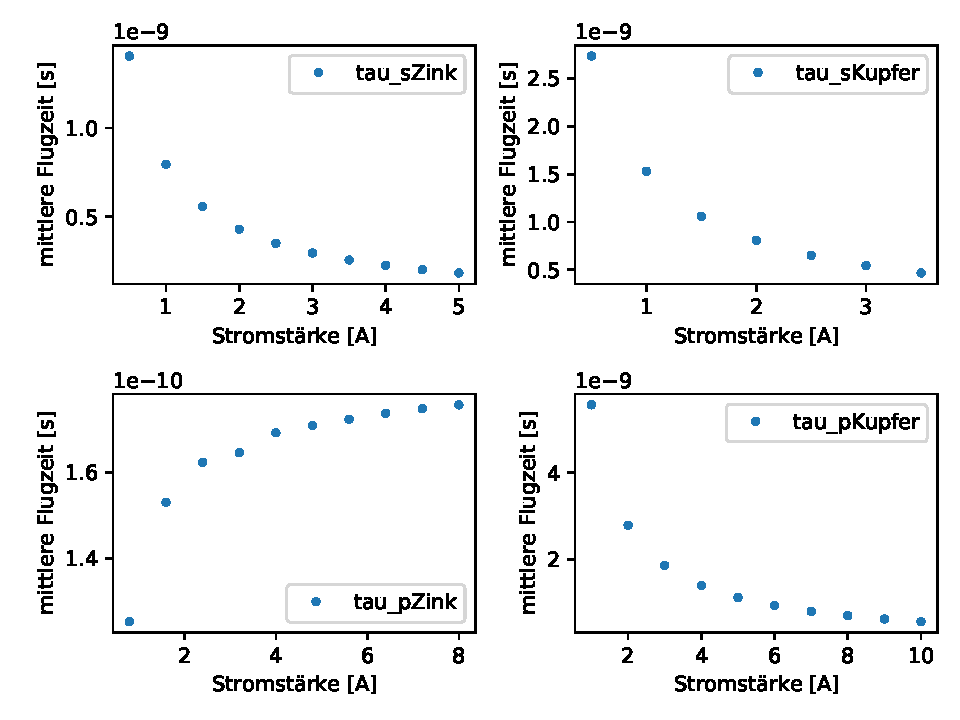
\includegraphics[width=1.1\textwidth]{build/tau.pdf}
        \caption{Ein Plot der mittleren Flugzeit gegen die Stromstärke.}
        \label{img:tau}
    \end{figure}


    \subsection{Mittlere Driftgeschwindigkeit}


    Die mittlere Driftgeschwindigkeit $\overline{v_d}$ berechnet sich aus:
    \begin{equation}
        \overline{v_d} = \frac{-n \cdot \symup{e_0}}{\symup{j}}
    \end{equation}
    mit der Stromdichte j = $\SI{1}{\ampere\per\milli\meter\squared}$.
    \noindent
    Einsetzten ergibt dann \ref{tab:Ergvd1},\ref{tab:Ergvd2}:
    \begin{figure}[H]
        \centering
        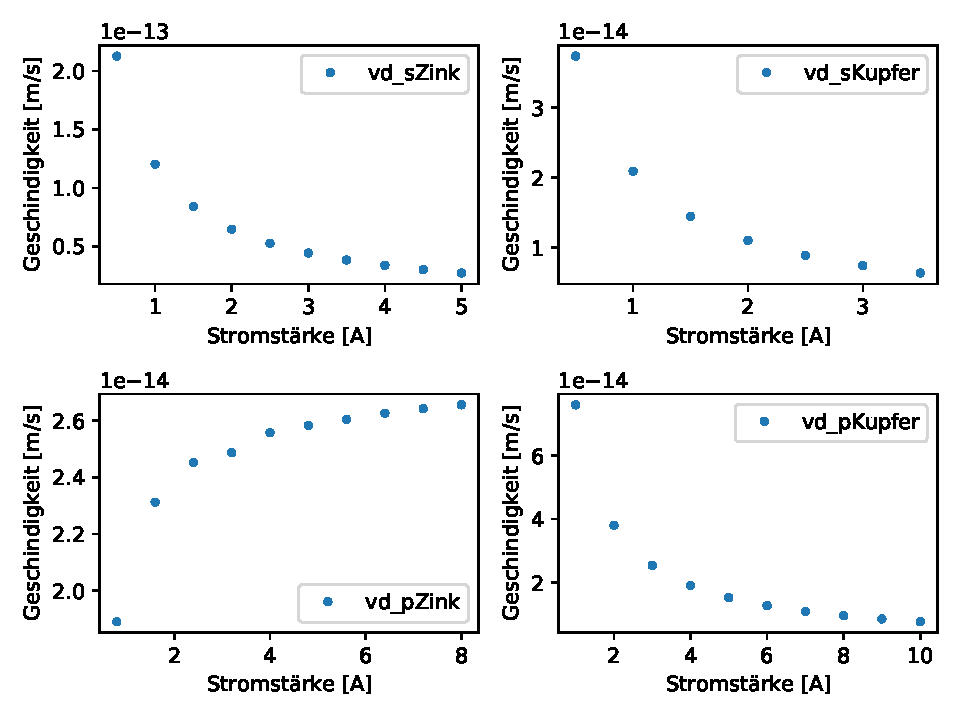
\includegraphics[width=1.1\textwidth]{build/Driftgeschwindigkeit.pdf}
        \caption{Ein Plot der Driftgeschwindigkeit gegen die Stromstärke.}
        \label{img:vd}
    \end{figure}


    \subsection{Beweglichkeit}


    Die Formel
    \begin{equation}
        \mu= -\frac{1}{2}\frac{\symup{e_0}}{\symup{m_0}}\cdot   \overline{\tau}
    \end{equation}
    stellt eine Beziehung zwischen $\overline{\tau}$ und $\mu$ auf. Mit den Werten für $\overline{\tau}$ \ref{tab:Ergtau1} berechnen sich nun folgende Werte 
    für $\overline{\mu}$ \ref{tab:ErgBew1},\ref{tab:ErgBew2}:

    \begin{figure}[H]
        \centering
        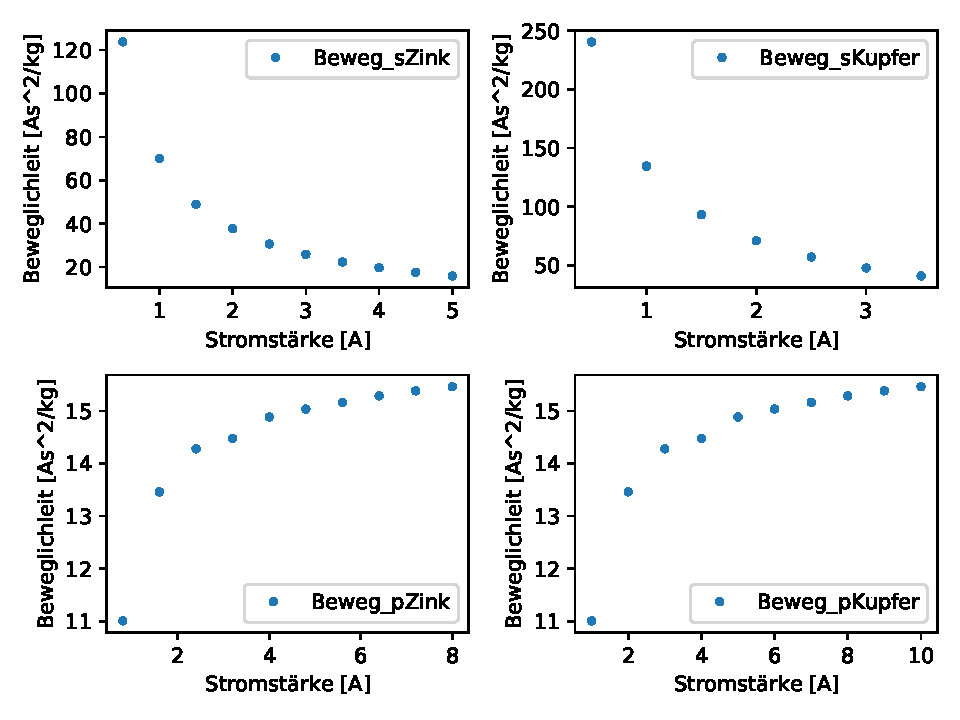
\includegraphics[width=1.1\textwidth]{build/Beweglichkeit.pdf}
        \caption{Ein Plot der Beweglichkeit gegen die Stromstärke.}
        \label{img:Beweg}
    \end{figure}


    \subsection{Totalgeschwindigkeit}


    Für die Totalgeschwindigkeit wird zunächst ein Wert für die Fermi-Energie berechnet werden, diese berechnet sich mittels der Formel:
    \begin{equation}
        E_F = \frac{\symup{h}^2}{2 \cdot \symup{m_0}}\sqrt{\left(\frac{3}{8\pi}\right)^2}
    \end{equation}
    Hier ist h das planksche Wirkungsquantum($\SI{6.626e-34}{\joule\second}$).
    Die Fermi-Energie berechnet sich zu: \ref{tab:ErgFE1},\ref{tab:ErgFE2}

    \begin{figure}[H]
        \centering
        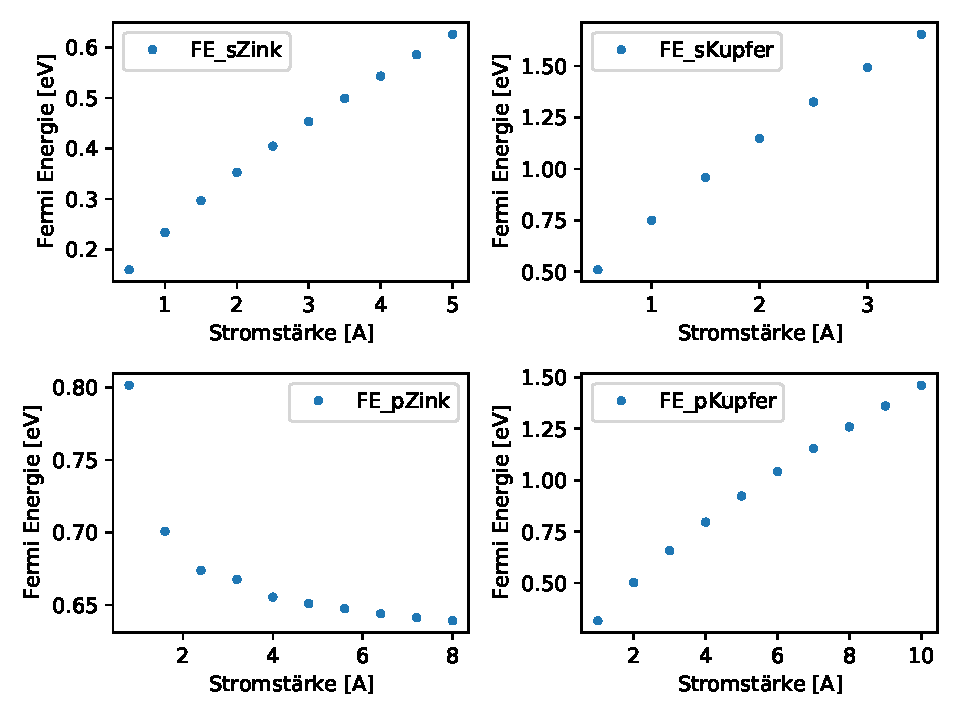
\includegraphics[width=1.1\textwidth]{build/Fermi.pdf}
        \caption{Ein Plot der Fermi-Energie gegen die Stromstärke.}
        \label{img:FE}
    \end{figure}

    Mittels der Fermi-Energie lässt sich nun über 

    \begin{equation}
        |\overline{v}| \approx \sqrt{\frac{2E_F}{\symup{m_0}}} \nonumber
    \end{equation}

    die Totalgeschwindigkeit bestimmen \ref{tab:ErgvT1},\ref{tab:vT2}: 

    \begin{figure}[H]
        \centering
        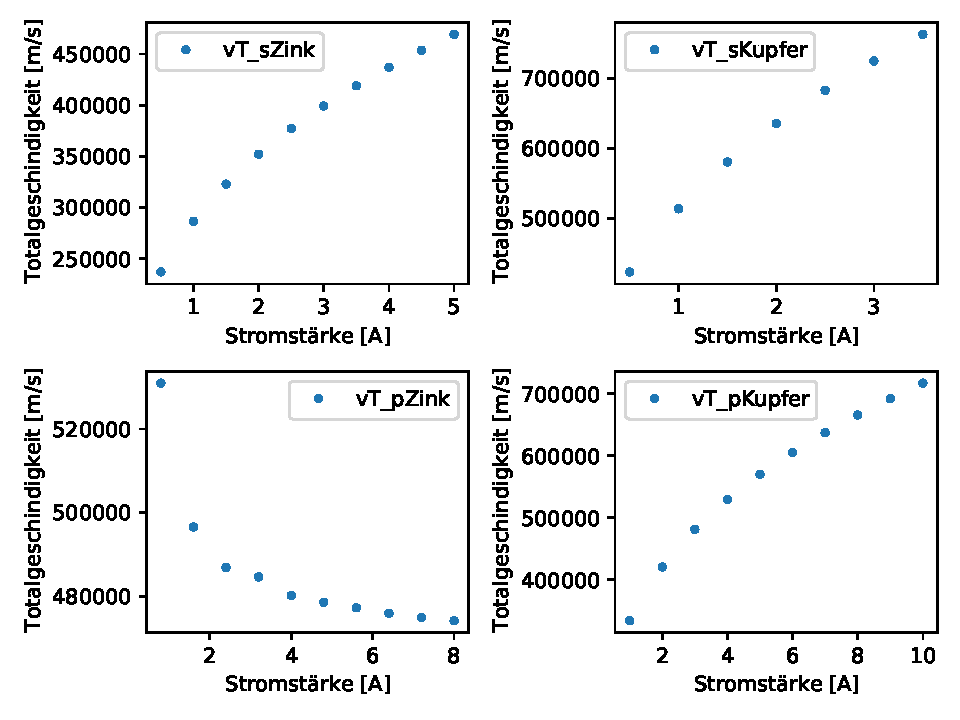
\includegraphics[width=1.1\textwidth]{build/Totalgeschwindigkeit.pdf}
        \caption{Ein Plot der Totalgeschwindigkeit gegen die Stromstärke.}
        \label{img:vT}
    \end{figure}


    \subsection{Mittlere freie Weglänge}


    Die mittlere freie Weglänge lässt sich nun mit der Totalgeschwindigkeit $|\overline{v}|$ und mittleren Flugzeit $\overline{\tau}$ berechnen:
    \begin{equation}
        \overline{l} \approx \overline{\tau} \cdot |\overline{v}| \nonumber
    \end{equation}

    
    \begin{figure}[H]
        \centering
        \includegraphics[width=1.1\textwidth]{build/mittlere_Weglänge.pdf}
        \caption{Ein Plot der mittleren freien Weglänge gegen die Stromstärke.}
        \label{img:mfl}
    \end{figure}
    \noindent
    Die Zahlenwerte zu den Plots befinden sich hier \ref{tab:ErgmW1},\ref{tab:ErgmW2}:

    \subsection{Elektronenleitung}
    Da von der Tatsache ausgegangen wird, dass Kupfer ein Elektronenleiter ist und bei Kupfer und Zink unterschiedliche Vorzeichen für
    die Hall-Spannung gemessen wurde, ist relativ sicher, dass bei Zink die Löcherleitung überwiegt.





















